%%%%%%%%%%%%%%%%%%%%% SEÇÃO GERENCIAMENTO
\chapter{Gerenciamento do Projeto}

Para o gerenciamento do projeto, nas Fases de Concepção e Detalhamento da Solução (01 e 02), foram planejados e documentados, de acordo com os planos estabelecidos pelo PMBOK \cite{pmbok}, as
áreas de Custos, Aquisições, Recursos Humanos e Riscos. A documentação dos planos podem ser visualizados nos apêndices do
\href{https://drive.google.com/file/d/0B5InkGKx6O-MR1B3eVYzZFpjQ3c/view?usp=sharing}{Relatório 1}.

A comunicação da equipe permaneceu como definida nas Fases 01 e 02 e na fase de Projeto e Construção da Solução, e o cronograma do projeto foi atualizado assim como as ferramentas de apoio utilizadas.

\section*{Ferramentas}

\textbf{WhatsApp}:
Aplicativo de mensagens para troca de informações que não necessitam de um encontro presencial.

\textbf{Google Drive\footnote{https://drive.google.com/}}: Serviço de armazenamento de arquivos utilizado para compartilhar todo o material gráfico (documentos, artigos, relatório, \textit{slides}, imagens e etc) utilizados para desenvolvimento do projeto.

\textbf{GitHub\footnote{https://github.com/}}: Ferramenta de gerenciamento de versões utilizada para armazenar e gerenciar
a escrita do relatório.

\section*{Estrutura Analítica de Projeto}

A EAP apresentada na Figura \ref{eap}, está dividida nas seguintes áreas: Planejamento do Projeto, Interface/Processamento, Eletroeletrônica, Eletromecânica, Estrutura e Encerramento do Projeto. O planejamento e o encerramento contemplam entregáveis relacionados ao projeto propriamente dito, e as demais áreas contemplam os entregáveis relacionados ao produto. As demais áreas foram estabelecidas de acordo com os módulos da bancada. Sendo:

\textbf{Interface/Processamento:} Módulo responsável por tratar da interação com o usuário da bancada, recebendo os parâmetros para controle da bancada e apresentando para o usuário os dados coletados no ensaio.

\textbf{Eletroeletrônica:} Módulo responsável por obter e tratar os sinais brutos dos sensores, disponibilizando dados para os demais módulos. Também é responsável pelo controle da vibração da mesa e interação com os motores.

\textbf{Eletromecânica:} Módulo responsável pelo acionamento do sistema por meio de motores de indução trifásicos, bem como controlar as velocidades e torques exigidos usando-se inversores de frequência afim de gerar a vibração na bancada definida pelo usuário.

\textbf{Estrutura:} Módulo responsável pelos cálculos/simulações estruturais, simulações modais, procura/aquisição dos materiais de construção e fabricação da bancada.

Para cada entregável foi colocado uma \textit{tag} indicando em que ponto de controle (entrega intermediária do projeto) deverá ser entregue, na qual:

\indent \textbf{PC1:} Ponto de Controle 1 - Concepção e Detalhamento da Solução

\indent \textbf{PC2:} Ponto de Controle 2 - Projeto e Construção da Solução

\indent \textbf{PC3:} Ponto de Controle 3 - Integração

\section*{Cronograma}

A partir dos entregáveis estabelecidos na EAP foram definidas as atividades e os prazos. Estes foram acordados entre os líderes de
cada área e considerando prazo total do projeto (19/08 a 02/12) e as entregas intermediárias (02/09, 04/11 e 30/11).
O cronograma do projeto de forma macro pode ser visto na Figura \ref{cronograma} e o seu detalhamento está disponível
no Google Drive \href{https://drive.google.com/file/d/0B28JW3Vcm0jLdElSSGNPcU4yVEU/view?usp=sharing}{(Cronograma)}.

Para a Fase 04 (Integração) do projeto optou-se por utilizar iterações, como previsto pelo
\textit{framework} Scrum \cite{scrum}.
As iterações tiveram duração aproximada de 1 semana,
nas quais as atividades foram planejadas no início da iteração de acordo
com a macro-atividade estabelecida no cronograma. O planejamento das iterações pode ser visto nas Tabelas \ref{tab:iteracao1},
\ref{tab:iteracao2}, \ref{tab:iteracao3}, \ref{tab:iteracao4} e \ref{tab:iteracao5}.

\begin{figure}[]
\centering
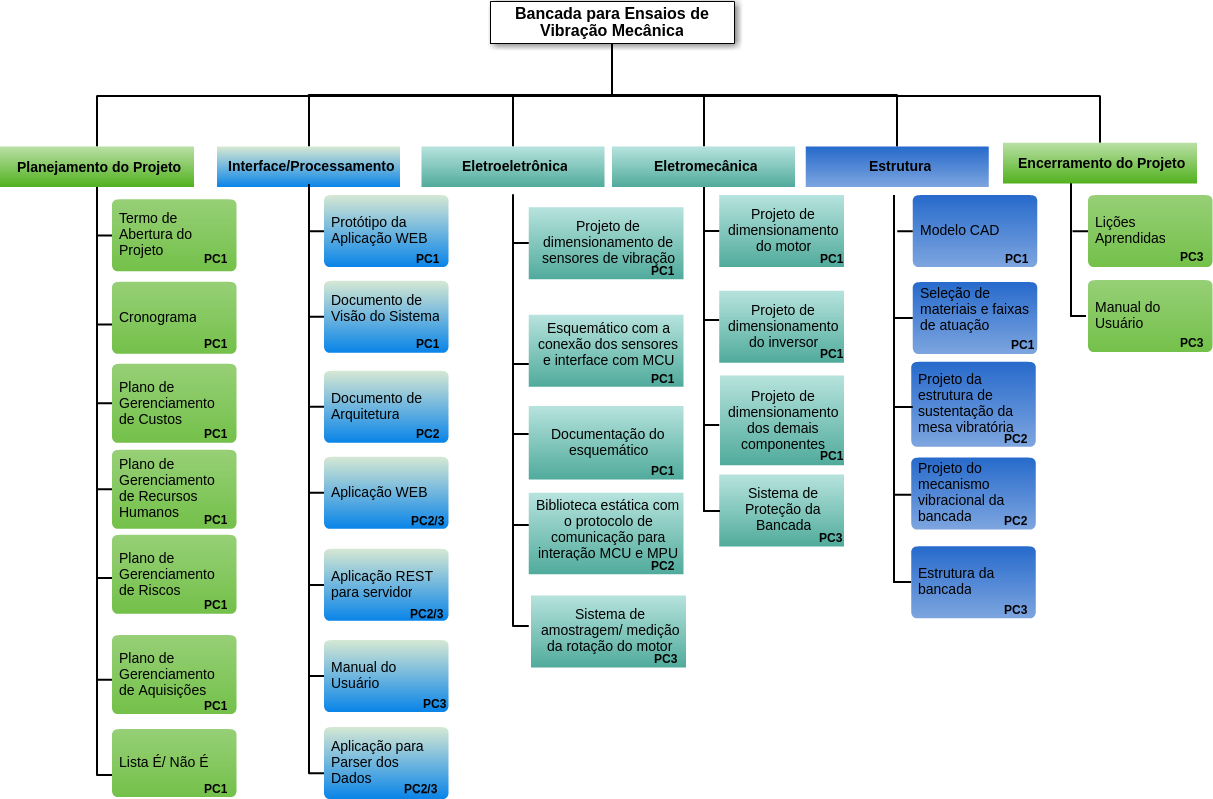
\includegraphics[keepaspectratio=true,scale=0.6,angle=90]{figuras/eap.png}
\caption{EAP do projeto}
\label{eap}
\end{figure}

\begin{figure}[H]
\centering
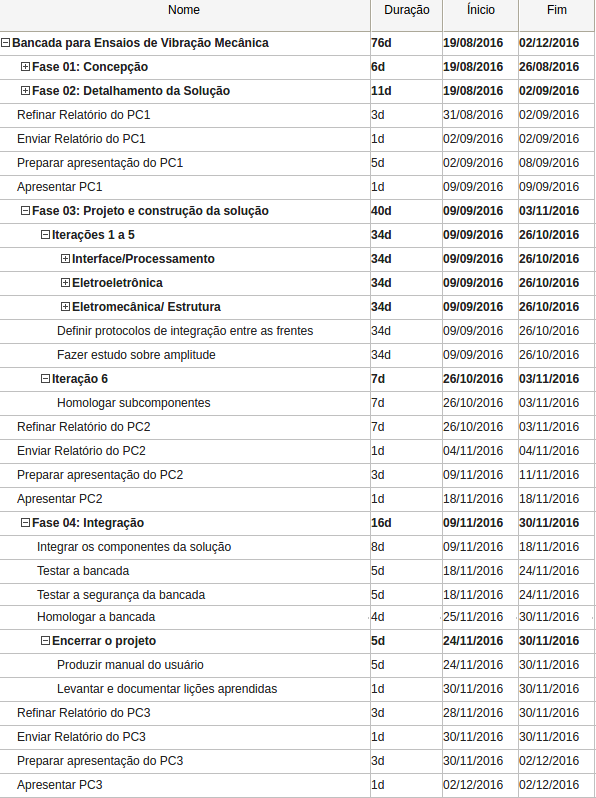
\includegraphics[scale=0.9]{figuras/cronograma_macro.png}
\caption{Cronograma do projeto}
\label{cronograma}
\end{figure}

%%%%%%%%%% ATUALIZAR CRONOGRAMA DAS ITEGRAÇÕES

\begin{table}[H]
\centering
\caption{Atividades - Iteração 6}
\label{tab:iteracao1}
\begin{tabular}{|l|l|}
\hline
\multicolumn{1}{|c|}{\textbf{Início da Iteração}} & \multicolumn{1}{c|}{04/11}                                                                                                                                                                                                                                        \\ \hline
\multicolumn{1}{|c|}{\textbf{Fim da Iteração}}    & \multicolumn{1}{c|}{11/11}                                                                                                                                                                                                                                        \\ \hline
\multicolumn{1}{|c|}{\textbf{Equipe}}             & \multicolumn{1}{c|}{\textbf{Atividades planejadas}}                                                                                                                                                                                                               \\ \hline
\textbf{Estrutura}                                & \begin{tabular}[c]{@{}l@{}}- Modelar mola com menos Rigidez\\ - Adquirir novas molas\end{tabular}                                                                                                                                                                                 \\ \hline
\textbf{Eletromecânica}                           & \begin{tabular}[c]{@{}l@{}}- Modelagem do sistema de proteção da bancada \\  - Comprar tomadas e cabos\end{tabular}                                                                                                                    \\ \hline
\textbf{Eletroeletrônica}                         & \begin{tabular}[c]{@{}l@{}}- Formalizar novo protocolo\\ - Modelar Circuito de Expansão\end{tabular}                                                             \\ \hline
\textbf{Interface/Processamento}                  & \begin{tabular}[c]{@{}l@{}}- Integrar aplicações Web e Server via REST\\ - Desenvolvimento do novo protocolo\end{tabular} \\ \hline
\end{tabular}
\end{table}

\begin{table}[H]
\centering
\caption{Atividades - Iteração 7}
\label{tab:iteracao1}
\begin{tabular}{|l|l|}
\hline
\multicolumn{1}{|c|}{\textbf{Início da Iteração}} & \multicolumn{1}{c|}{11/11}                                                                                                                                                                                                                                        \\ \hline
\multicolumn{1}{|c|}{\textbf{Fim da Iteração}}    & \multicolumn{1}{c|}{18/11}                                                                                                                                                                                                                                        \\ \hline
\multicolumn{1}{|c|}{\textbf{Equipe}}             & \multicolumn{1}{c|}{\textbf{Atividades planejadas}}                                                                                                                                                                                                               \\ \hline
\textbf{Estrutura}                                & \begin{tabular}[c]{@{}l@{}}- Definicação e compra da correia de giro do eixo\\ - Modelagem do eixo desbalanceado\end{tabular}                                                                                                                                                                                 \\ \hline
\textbf{Eletromecânica}                           & \begin{tabular}[c]{@{}l@{}}- Construção do sistema de proteção da bancada \\ - Ajuste do inversor com o sistema de proteção\end{tabular}                                                                                                                    \\ \hline
\textbf{Eletroeletrônica}                         & \begin{tabular}[c]{@{}l@{}}- Modelagem do circuito de controle do motor \\ - Modelagem do circuito de controle e recebimento  \\ de dados dos sensores \end{tabular}                                                             \\ \hline
\textbf{Interface/Processamento}                  & \begin{tabular}[c]{@{}l@{}}- Desenvolvimento do método de processamento de dados \\ - Integração dos dados da simulação para \\ a plotagem dos dados nos gráficos \\ - Serialização JSON dos resultados do servidor para \\ aplicação Web e parser para o banco de dados da aplicação Web\end{tabular} \\ \hline
\end{tabular}
\end{table}

\begin{table}[H]
\centering
\caption{Atividades - Iteração 8}
\label{tab:iteracao1}
\begin{tabular}{|l|l|}
\hline
\multicolumn{1}{|c|}{\textbf{Início da Iteração}} & \multicolumn{1}{c|}{18/11}                                                                                                                                                                                                                                        \\ \hline
\multicolumn{1}{|c|}{\textbf{Fim da Iteração}}    & \multicolumn{1}{c|}{25/11}                                                                                                                                                                                                                                        \\ \hline
\multicolumn{1}{|c|}{\textbf{Equipe}}             & \multicolumn{1}{c|}{\textbf{Atividades planejadas}}                                                                                                                                                                                                               \\ \hline
\textbf{Estrutura}                                & \begin{tabular}[c]{@{}l@{}}- Construção da massa desbalanceada\\ - Adaptação do mancal de acordo \\ com a nova massa desbalanceada\end{tabular}                                                                                                                                                                                 \\ \hline
\textbf{Eletromecânica}                           & \begin{tabular}[c]{@{}l@{}}- Construção de pulpito para colocar sistema de proteção \end{tabular}                                                                                                                    \\ \hline
\textbf{Eletroeletrônica}                         & \begin{tabular}[c]{@{}l@{}}- Modelagem do circuito de alimentação \\ - Desenvolvimento do protocolo de comunicação\end{tabular}                                                             \\ \hline
\textbf{Interface/Processamento}                  & \begin{tabular}[c]{@{}l@{}}- Refatoração da interface do usuário \\ - Criação da Timeline do experimento \\ - Desenvolvimento de gráficos por job\end{tabular} \\ \hline
\end{tabular}
\end{table}

\begin{table}[H]
\centering
\caption{Atividades - Iteração 9}
\label{tab:iteracao1}
\begin{tabular}{|l|l|}
\hline
\multicolumn{1}{|c|}{\textbf{Início da Iteração}} & \multicolumn{1}{c|}{25/11}                                                                                                                                                                                                                                        \\ \hline
\multicolumn{1}{|c|}{\textbf{Fim da Iteração}}    & \multicolumn{1}{c|}{02/11}                                                                                                                                                                                                                                        \\ \hline
\multicolumn{1}{|c|}{\textbf{Equipe}}             & \multicolumn{1}{c|}{\textbf{Atividades planejadas}}                                                                                                                                                                                                               \\ \hline
\textbf{Estrutura}                                & \begin{tabular}[c]{@{}l@{}}- Ajuste do tampo\\ - Ajuste do mancal e eixo desbalanceado\end{tabular}                                                                                                                                                                                 \\ \hline
\textbf{Eletromecânica}                           & \begin{tabular}[c]{@{}l@{}}- Instalação dos fusíveis \\ - Instalação do sistema de proteção no Pulpito \\ \end{tabular}                                                                                                                    \\ \hline
\textbf{Eletroeletrônica}                         & \begin{tabular}[c]{@{}l@{}}- Construção do circuito de alimentação \\ - Construção do circuito de expansão \\ - Construção do circuito de controle do motor \\ - Construção do circuito de controle dos sensores\end{tabular}                                                             \\ \hline
\textbf{Interface/Processamento}                  & \begin{tabular}[c]{@{}l@{}}- Desenvolvimento de testes \\ de integração do sistema como um todoa\end{tabular} \\ \hline
\end{tabular}
\end{table}


% \begin{table}[H]
% \centering
% \caption{Atividades - Iteração 2}
% \label{tab:iteracao2}
% \begin{tabular}{|l|l|}
% \hline
% \multicolumn{1}{|c|}{\textbf{Início da Iteração}} & \multicolumn{1}{c|}{21/09}                                                                                                                            \\ \hline
% \multicolumn{1}{|c|}{\textbf{Fim da Iteração}}    & \multicolumn{1}{c|}{28/09}                                                                                                                            \\ \hline
% \multicolumn{1}{|c|}{\textbf{Equipe}}             & \multicolumn{1}{c|}{\textbf{Atividades planejadas}}                                                                                                   \\ \hline
% \textbf{Estrutura}                                & \begin{tabular}[c]{@{}l@{}}- Definir material da mesa e espessura\\ - Estimar os pesos\\ - Fazer cálculos estruturais\end{tabular}                    \\ \hline
% \textbf{Eletromecânica}                           & - Fazer sistema de acionamento do motor                                                                                                               \\ \hline
% \textbf{Eletroeletrônica}                         & \begin{tabular}[c]{@{}l@{}}- Trabalhar na estabilidade do módulo UART\\ - Trabalhar na arquitetura do módulo de sensoriamento\end{tabular} \\ \hline
% \textbf{Interface/Processamento}                  & \begin{tabular}[c]{@{}l@{}}- Implementar início do experimento\\ - Implementar timer do experimento\\ - Implementar captura dos sensores\end{tabular} \\ \hline
% \end{tabular}
% \end{table}

% \begin{table}[H]
% \centering
% \caption{Atividades - Iteração 3}
% \label{tab:iteracao3}
% \begin{tabular}{|l|l|}
% \hline
% \multicolumn{1}{|c|}{\textbf{Início da Iteração}} & \multicolumn{1}{c|}{28/09}                                                                                                                                                                                                                  \\ \hline
% \multicolumn{1}{|c|}{\textbf{Fim da Iteração}}    & \multicolumn{1}{c|}{12/10}                                                                                                                                                                                                                  \\ \hline
% \multicolumn{1}{|c|}{\textbf{Equipe}}             & \multicolumn{1}{c|}{\textbf{Atividades planejadas}}                                                                                                                                                                                         \\ \hline
% \textbf{Estrutura}                                & \begin{tabular}[c]{@{}l@{}}- Comprar pés\\ - Furar fixação do motor\\ - Fixar apoio dos pés e molas\end{tabular}                                                                                                                            \\ \hline
% \textbf{Eletromecânica}                           & - Programar inversor trifásico                                                                                                                                                                                                              \\ \hline
% \textbf{Eletroeletrônica}                         & \begin{tabular}[c]{@{}l@{}}- Finalizar módulo UART do BSP \\ - Finalizar conversor PWM-DC\end{tabular} \\ \hline
% \textbf{Interface/Processamento}                  & \begin{tabular}[c]{@{}l@{}}- Adaptar parser para prover escalabilidade\\ - Implementar rotina de verificação e passagem\\ dos dados da porta serial \\ - Implementar visualização dos ensaios realizados \end{tabular} \\ \hline
% \end{tabular}
% \end{table}

% \begin{table}[H]
% \centering
% \caption{Atividades - Iteração 4}
% \label{tab:iteracao4}
% \begin{tabular}{|l|l|}
% \hline
% \multicolumn{1}{|c|}{\textbf{Início da Iteração}} & \multicolumn{1}{c|}{14/10}                                                                                                                                                           \\ \hline
% \multicolumn{1}{|c|}{\textbf{Fim da Iteração}}    & \multicolumn{1}{c|}{21/10}                                                                                                                                                           \\ \hline
% \multicolumn{1}{|c|}{\textbf{Equipe}}             & \multicolumn{1}{c|}{\textbf{Atividades planejadas}}                                                                                                                                  \\ \hline
% \textbf{Estrutura}                                & \begin{tabular}[c]{@{}l@{}}- Comprar e instalar molas\\ - Projetar o retentor da correia\\ - Analisar o tampo com os reforços\\ - Fixar o motor\end{tabular}                         \\ \hline
% \textbf{Eletromecânica}                           & \begin{tabular}[c]{@{}l@{}}- Fazer teste de integração\\ - Fazer sistema de proteção\\ - Estudar a amplitude \\ - Fixar o motor\end{tabular}                                                            \\ \hline
% \textbf{Eletroeletrônica}                         & \begin{tabular}[c]{@{}l@{}}- Testar layouts de controle do inversor\\ - Finalizar BSP\\ - Estudar obtenção da frequência * crítico\\ - Estudar viabilidade da amplitude\end{tabular} \\ \hline
% \textbf{Interface/Processamento}                  & \begin{tabular}[c]{@{}l@{}}- Integrar aplicação WEB com o servidor\\ - Implementar população do banco da aplicação\\ - Implementar mais testes \\ - Fazer documento de arquitetura \end{tabular}                          \\ \hline
% \end{tabular}
% \end{table}

% \begin{table}[H]
% \centering
% \caption{Atividades - Iteração 5}
% \label{tab:iteracao5}
% \begin{tabular}{|l|l|}
% \hline
% \multicolumn{1}{|c|}{\textbf{Início da Iteração}} & \multicolumn{1}{c|}{21/10}                                                                                                                                                                                                                                                                                         \\ \hline
% \multicolumn{1}{|c|}{\textbf{Fim da Iteração}}    & \multicolumn{1}{c|}{28/10}                                                                                                                                                                                                                                                                                         \\ \hline
% \multicolumn{1}{|c|}{\textbf{Equipe}}             & \multicolumn{1}{c|}{\textbf{Atividades planejadas}}                                                                                                                                                                                                                                                                \\ \hline
% \textbf{Estrutura}                                & \begin{tabular}[c]{@{}l@{}}- Cortar chapas para produção dos copinhos\\ - Furar chapas\\ - Usinar os copinhos\\ - Cortar copinhos usinados\\ - Soldar copinhos na chapa\\ - Soldar chapa na estrutura\\ - Usinar coroa da polia\end{tabular}                                                                       \\ \hline
% \textbf{Eletromecânica}                           & \begin{tabular}[c]{@{}l@{}}- Montar cabeamento do inversor\\ - Montar cabeamento do motor\end{tabular}                                                                                                                                                                                                             \\ \hline
% \textbf{Eletroeletrônica}                         & \begin{tabular}[c]{@{}l@{}}- Finalizar circuito de contagem de unidades \\ de expansão\\ - Fechar módulo I2C do BSP\end{tabular}                                                                                                                                                                                   \\ \hline
% \textbf{Interface/Processamento}                  & \begin{tabular}[c]{@{}l@{}}- Concluir fluxo de ida e de volta da aplicação\\       - Ler sensores e dados dos sensores\\ - Implementar pausa do ensaio a cada mudança de \\ frequência\\ - Adaptar modelagem do banco do REST\\ - Definir técnica de processamento dos dados\\ - Otimizar a aplicação\end{tabular} \\ \hline
% \end{tabular}
% \end{table}

\newpage
\section{Acompanhamento das Aquisições}

Na Tabela \ref{tab:acompanhamento_custos} podem ser vistas as aquisições realizadas durante a Fase 03 do projeto.

%%%% ATUALIZAR PLANILHA DE CUSTOS %%%%%%%%%%

\begin{table}[H]
\centering
\begin{tabular}{|l|c|l|}
\hline
\multicolumn{1}{|c|}{\textbf{Item adquirido}} & \textbf{Quantidade} & \multicolumn{1}{c|}{\textbf{Custo Unitário}} \\ \hline
Inversor trifásico                                          & 1                & R\$ 400,00                           \\ \hline
4m de cabo de 5 polos                                 & 1                & R\$ 15,00                             \\ \hline
1 tomada stack 3f+n+t 32a                         & 1                & R\$ 35,00                             \\ \hline
1 tomada stack 3f+n+t 16a macho (plug)  & 1                 & R\$ 20,00                             \\ \hline
1 tomada stack 3f+n+t 16a fêmea             & 1                 & R\$ 20,00                             \\ \hline
4m de cabo de 4 polos 3f+t                         & 1                 & R\$ 15,00                             \\ \hline
Terminais pré-isolados                                 & 10               & R\$ 5,00                                \\ \hline
Acelerômetro adxl335 triaxial                      & 6                 & R\$ 19,55                              \\ \hline
Solda                                                              & 1                 & R\$ 250,00                            \\ \hline
Tampo                                                           & 1                  & R\$ 170,00                           \\ \hline
Gasolina                                                        & 10L              & R\$ 35,00                             \\ \hline
Pés                                                                 & 4                 & R\$ 69,00                             \\ \hline
Molas                                                             & 4                 & R\$ 11,00                              \\ \hline
Parafusos                                                       & 8                 & R\$ 7,00                                \\ \hline
Cantoneira                                                     & 1                 & R\$ 170,00                             \\ \hline
Polia                                                               & 1                 & R\$ 10,00                              \\ \hline
\multicolumn{2}{|c|}{\textbf{Orçamento}}                      & R\$ 1.347.00                         \\ \hline
\multicolumn{2}{|c|}{\textbf{Custo total}}                      & R\$ 1.251,55                          \\ \hline
\end{tabular}
\caption{Aquisições do projeto até o Final de PC2 - Fonte: Autores}
\label{tab:acompanhamento_custos}
\end{table}

Na Tabela \ref{tab:acompanhamento_custos_1} podem ser vistas as aquisições realizadas durante a Fase 04 do projeto.

\begin{table}[H]
\centering
\begin{tabular}{|l|c|l|}
\hline
\multicolumn{1}{|c|}{\textbf{Item adquirido}} & \textbf{Quantidade} & \multicolumn{1}{c|}{\textbf{Custo Unitário}} \\ \hline
Molas com Rigidez equilibrada                                          & 4                & R\$ 40,00                           \\ \hline
Porcas e Parafusos                                                             & 5                & R\$ 2,50                            \\ \hline
Polia da Massa Desbalanceada                                          & 1               & R\$ 75,00                           \\ \hline
Tinta Spray                                                                          & 4                & R\$ 75,00                         \\ \hline
\multicolumn{2}{|c|}{\textbf{Orçamento}}                      & R\$ 1.347.00                         \\ \hline
\multicolumn{2}{|c|}{\textbf{Custo total}}                      & R\$                           \\ \hline
\end{tabular}
\caption{Aquisições do projeto até o Final de PC3 - Fonte: Autores}
\label{tab:acompanhamento_custos_1}
\end{table}

%%%%%%%%%%%%%%%%%%%%% FIM SEÇÃO GERENCIAMENTO